\documentclass[a4paper,12pt]{article}
\usepackage{iftex}
\ifPDFTeX
  \usepackage[T5,T1]{fontenc}
  \usepackage{mathptmx}
\else
  \usepackage{fontspec}
  \defaultfontfeatures{Ligatures=TeX}
  \setmainfont{Times New Roman}
  \setsansfont{Times New Roman}
  \IfFontExistsTF{Consolas}{%
    \setmonofont{Consolas}[Scale=0.84]
  }{%
    \setmonofont{Courier New}[Scale=0.86]
  }
\fi
\usepackage[vietnamese]{babel}
\ifPDFTeX
  \usepackage{microtype}
\else
  \usepackage[protrusion=true,expansion=false]{microtype}
\fi
\sloppy
\emergencystretch=4em
\tolerance=2500
\hbadness=10000
\hfuzz=1.5pt
\vfuzz=2.0pt
\raggedbottom
\usepackage{amsmath}
\usepackage{indentfirst}
\usepackage{geometry}
\geometry{a4paper, top=20mm, bottom=20mm, left=30mm, right=20mm, headheight=15pt, headsep=10mm, footskip=10mm}
\usepackage{setspace}
\setstretch{1.15}
\usepackage{booktabs,tabularx,array,multirow}
\usepackage{ragged2e}
\renewcommand{\tabularxcolumn}[1]{>{\RaggedRight\arraybackslash\hspace{0pt}}p{#1}}
\newcolumntype{Y}{>{\Centering\arraybackslash\hspace{0pt}}X}
\newcolumntype{L}[1]{>{\RaggedRight\arraybackslash\hspace{0pt}}p{#1}}
\newcolumntype{C}[1]{>{\Centering\arraybackslash\hspace{0pt}}p{#1}}
\usepackage{graphicx,float}
\usepackage{fancyhdr}
\usepackage[unicode, colorlinks=false, pdfborder={0 0 0}]{hyperref}

\pagestyle{fancy}
\fancyhf{}
\fancyhead[L]{\fontsize{11pt}{13pt}\itshape\selectfont Báo cáo Tóm tắt Đồ án tốt nghiệp Đại học}
\fancyhead[R]{\fontsize{11pt}{13pt}\itshape\selectfont Nhóm Thanh\_01 (A06) -- D22CQAT01-N}
\fancyfoot[L]{\fontsize{11pt}{13pt}\itshape\selectfont Nguyễn Văn An, Lê Đình Nghĩa -- D22CQAT01-N}
\fancyfoot[R]{\fontsize{11pt}{13pt}\selectfont \thepage}
\renewcommand{\footrulewidth}{0.4pt}

\setlength{\parskip}{3pt}
\setlength{\parindent}{15pt}

\begin{document}

\begin{center}
  {\bfseries\fontsize{13pt}{16pt}\selectfont HỌC VIỆN CÔNG NGHỆ BƯU CHÍNH VIỄN THÔNG}\\
  {\bfseries\fontsize{13pt}{16pt}\selectfont CƠ SỞ TẠI THÀNH PHỐ HỒ CHÍ MINH}\\
  {\bfseries\fontsize{13pt}{16pt}\selectfont KHOA CÔNG NGHỆ THÔNG TIN 2}\\
  \textbf{-----------------------------------------}\\[0.5cm]
  {\bfseries\fontsize{18pt}{22pt}\selectfont BÁO CÁO TÓM TẮT ĐỒ ÁN TỐT NGHIỆP}\\[0.4cm]
\end{center}

\section{Thông tin chung về Đồ án tốt nghiệp}

\begin{itemize}
    \item \textbf{1. Tên đồ án tốt nghiệp:} \textbf{``Nghiên cứu và xây dựng cơ chế Guardrails đa lớp cho hệ thống RAG doanh nghiệp trước tấn công Prompt Injection và rò rỉ dữ liệu nhạy cảm''}
    \item \textbf{2. Nhóm sinh viên thực hiện (Nhóm Thanh\_01 / A06):}
    \begin{itemize}
        \item Sinh viên 1 (Nhóm trưởng) --- Mã sinh viên: \textbf{N22DCAT001} \quad Họ và tên: \textbf{Nguyễn Văn An} \quad Lớp: \textbf{D22CQAT01-N}
        \item Sinh viên 2 --- Mã sinh viên: \textbf{N22DCAT038} \quad Họ và tên: \textbf{Lê Đình Nghĩa} \quad Lớp: \textbf{D22CQAT01-N}
    \end{itemize}
    \item \textbf{3. Giáo viên hướng dẫn:} \textbf{ThS. Nguyễn Hoàng Thành}
    \item \textbf{4. Ngành đào tạo:} \textbf{An toàn thông tin}
\end{itemize}

\section{Mục tiêu và cấu trúc của Đồ án tốt nghiệp}

\subsection{Mục tiêu của Đồ án tốt nghiệp}
Đồ án tốt nghiệp hướng tới giải quyết bài toán bảo vệ các hệ thống sinh văn bản tăng cường truy hồi (RAG), truy vấn cơ sở dữ liệu bằng ngôn ngữ tự nhiên (Text-to-SQL) và tác tử đa công cụ (Multi-Tool Agent) trước các đòn tấn công chèn chỉ dẫn trực tiếp/gián tiếp (Direct/Indirect Prompt \& SQL Injection) và rò rỉ dữ liệu nhạy cảm tại thời điểm chạy, đồng thời khắc phục triệt để hạn chế ``đánh giá khép kín'' thông qua bốn mục tiêu cụ thể:
\begin{enumerate}
    \item Thiết kế và hiện thực khung bảo mật đa lớp \textbf{Shield AI} kết hợp tầng tiền giải mã (\emph{Payload De-obfuscation Pre-decoder} cho Base64/ROT13/Leetspeak/Unicode), chuỗi Guard tất định (Input Guard, Provenance Guard, RAG Context Guard, Output/DLP Guard), bộ phán đoán ngữ nghĩa cục bộ (\emph{Semantic Judge} \texttt{gemma4:e2b-\allowbreak it-\allowbreak q4\_\allowbreak K\_\allowbreak M}) và kiểm soát truy cập trước truy hồi (\emph{Pre-retrieval RBAC}) trên nền truy hồi lai vectorized.
    \item Mở rộng kiến trúc bảo vệ sang dữ liệu có cấu trúc và tác tử đa công cụ: xây dựng \textbf{SQL Guard} dùng chính trình biên dịch \texttt{EXPLAIN} và \texttt{Authorizer AST callback} của SQLite để phân quyền tới từng bảng/cột, \textbf{Indirect Data-Cell Result Guard} quét từng ô dữ liệu trả về từ CSDL, và \textbf{Multi-Tool Company Agent} có hàng chờ phê duyệt cấp quản lý (\emph{Leader Approval Queue}).
    \item Đo đạc đầy đủ phân vị độ trễ \textbf{\texttt{p50 / p95 / p99}} của từng tầng xử lý khi bật và tắt Semantic Judge.
    \item Kiểm chứng độc lập trên benchmark công khai \textbf{\texttt{deepset/\allowbreak prompt-\allowbreak injections}} ($662$ mẫu), bắn trực tiếp công cụ red-team \textbf{\texttt{NVIDIA garak v0.\allowbreak 17.\allowbreak 1}} ($2.048$ probe HTTP REST) và \textbf{\texttt{PyRIT}} Converter/Adaptive Multi-Turn vào API sống, đồng thời đối sánh định lượng với \textbf{Meta Llama Guard~3 1B} và \textbf{NVIDIA NeMo Guardrails}.
\end{enumerate}

\subsection{Cấu trúc quyển Đồ án tốt nghiệp}
Ngoài phần Mở đầu, Kết luận, Tài liệu tham khảo và 4 Phụ lục, nội dung chính của quyển Đồ án tốt nghiệp (58 trang) được tổ chức thành 4 chương:
\begin{itemize}
    \item \textbf{Chương 1 --- Tổng quan về bài toán và cơ sở lý thuyết:} Phân tích kiến trúc RAG/Text-to-SQL/Agent, bề mặt tấn công theo OWASP LLM Top~10, nguyên lý phòng thủ chiều sâu và định vị Shield AI so với Llama Guard~3 \& NeMo Guardrails.
    \item \textbf{Chương 2 --- Phân tích yêu cầu và thiết kế hệ thống:} Đặc tả yêu cầu chức năng (FR-IN, FR-CTX, FR-OUT, FR-RAG, FR-SQL, FR-AGT, FR-LOG), yêu cầu phi chức năng, kiến trúc truy hồi lai vectorized và kiến trúc phòng thủ 9 bước cho Multi-Tool Agent \& Text-to-SQL.
    \item \textbf{Chương 3 --- Xây dựng và triển khai hệ thống:} Chi tiết hiện thực tầng tiền giải mã \texttt{\_\allowbreak expand\_\allowbreak deobfuscated\_\allowbreak views()}, bộ luật cấu trúc đa ngôn ngữ, tối ưu \texttt{think=False} cho Semantic Judge, SQLite Authorizer AST Guard và bộ kiểm thử tự động tích hợp ($469$ unit/integration tests).
    \item \textbf{Chương 4 --- Kiểm thử và đánh giá kết quả:} Trình bày thực nghiệm trả lời 5 câu hỏi nghiên cứu (CH1--CH5) trên hơn $3.200$ mẫu và probe kiểm thử.
\end{itemize}

\section{Nội dung thực hiện và Kết quả đạt được}

\subsection{Kiến trúc phòng thủ chiều sâu cho RAG, Text-to-SQL và Multi-Tool Agent}

\begin{figure}[!htbp]
\centering
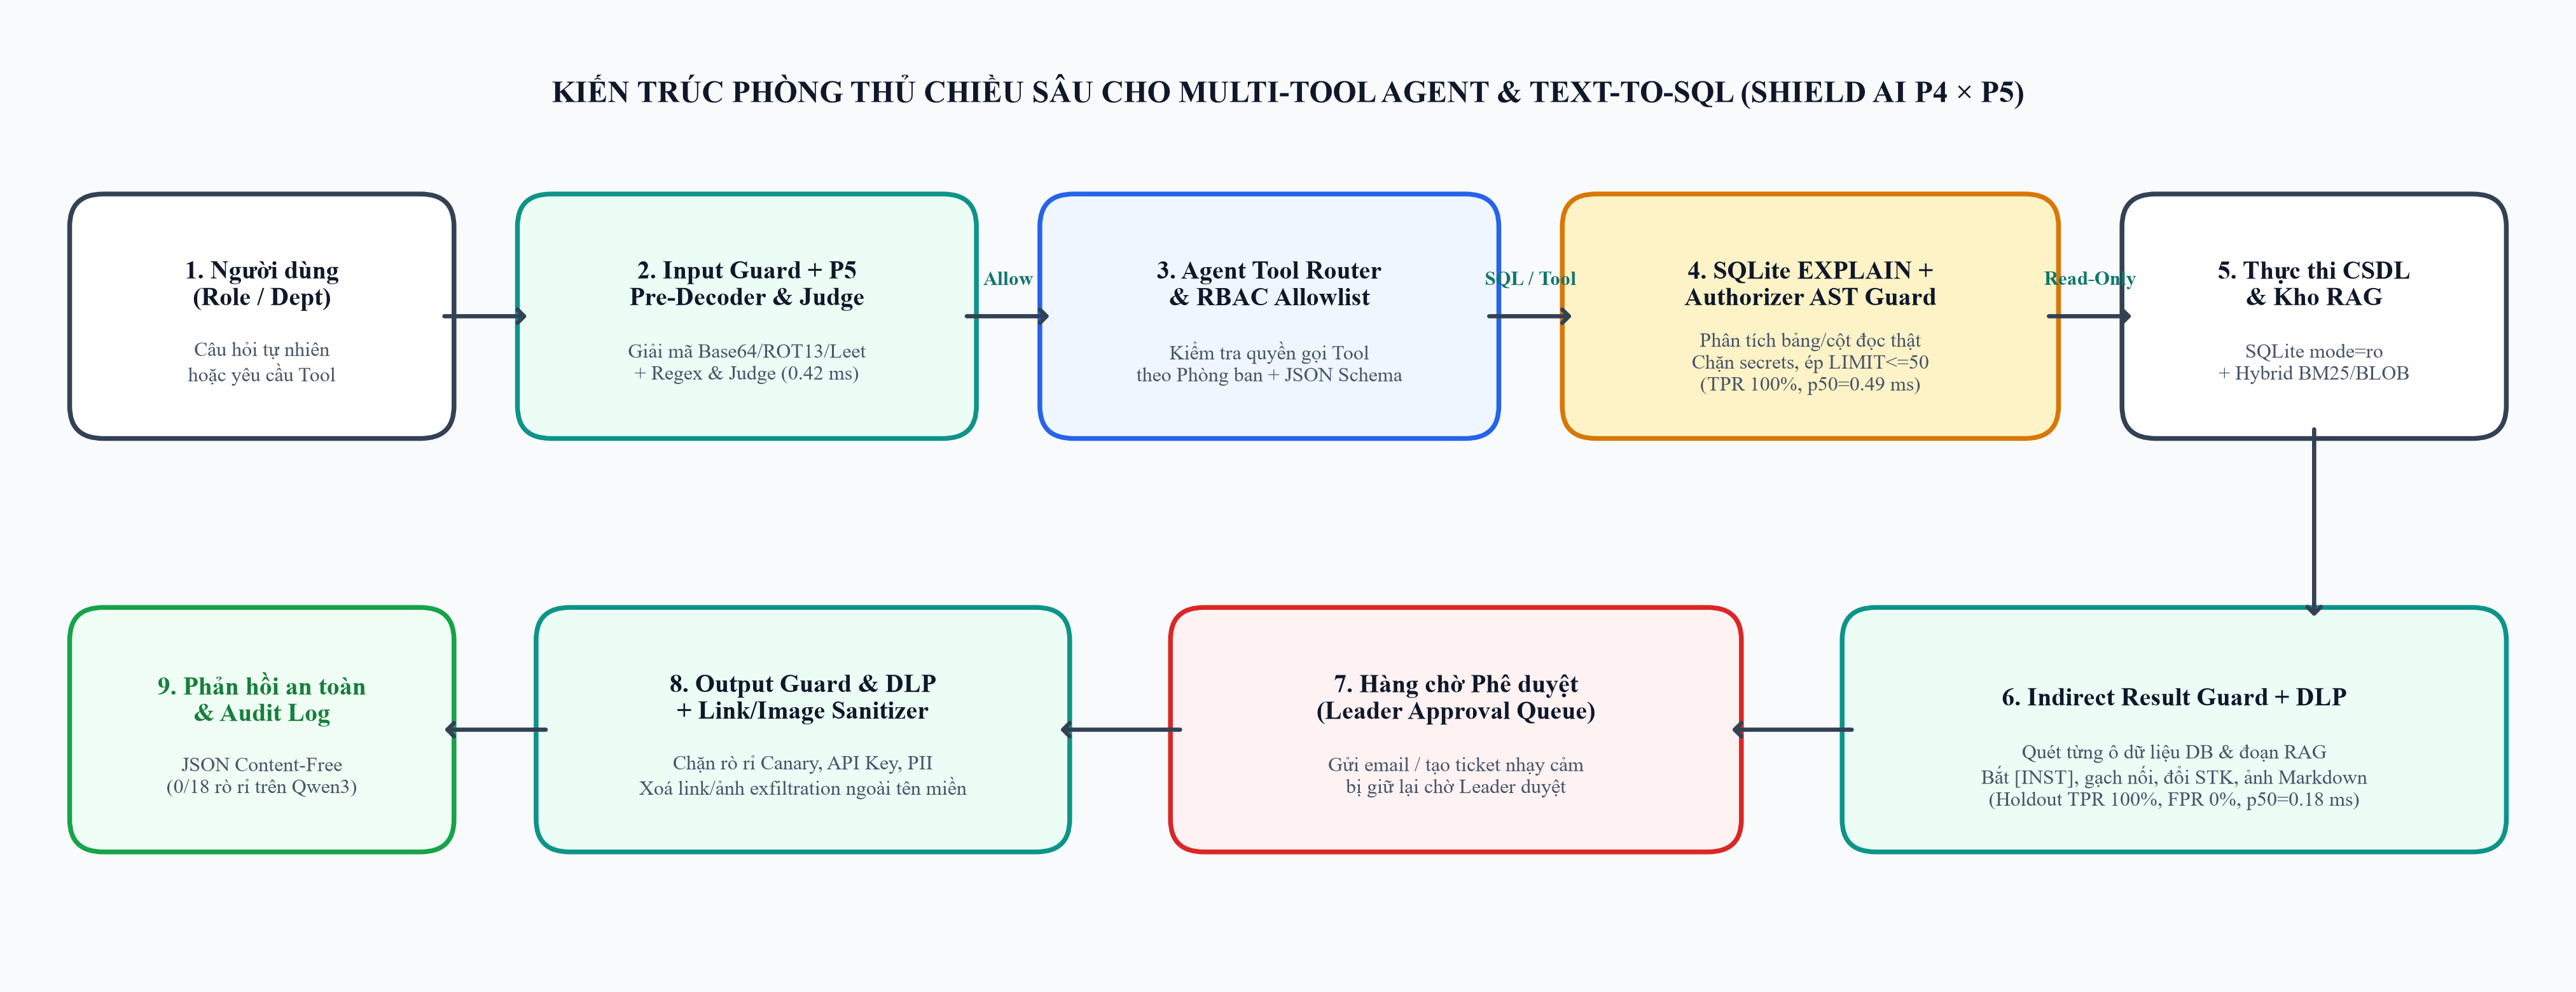
\includegraphics[width=0.96\linewidth]{figures/fig-sql-agent-architecture.png}
\caption{Kiến trúc phòng thủ chiều sâu 9 bước của Shield AI cho RAG, Text-to-SQL và Multi-Tool Agent}
\end{figure}

Hệ thống \textbf{Shield AI} bảo vệ toàn diện cả kho tài liệu không cấu trúc (48 tài liệu doanh nghiệp) lẫn cơ sở dữ liệu quan hệ (12 bảng SQL của doanh nghiệp nội thất Nhà Mộc Việt với $1.500$ đơn hàng, $84$ nhân sự, bảng mật \texttt{internal\_\allowbreak secrets}) thông qua:
\begin{itemize}
    \item \textbf{Tầng tiền giải mã (\emph{Payload Pre-decoder}) \& Input Guard:} Chuẩn hoá Unicode NFKC, loại bỏ ký tự ẩn zero-width, gấp đồng hình Cyrillic, giải nhiễu Leetspeak và tự động giải mã các khối Base64/ROT13 trước khi đối chiếu với bộ luật cấu trúc đa ngôn ngữ (Việt/Anh/Đức/Tây Ban Nha).
    \item \textbf{Pre-retrieval RBAC \& SQLite Authorizer AST Guard:} Áp phân quyền vai trò/phòng ban ngay trước bước truy hồi tài liệu và dùng chính trình biên dịch \texttt{EXPLAIN} + \texttt{sqlite3.\allowbreak set\_\allowbreak authorizer} của SQLite để kiểm tra mọi bảng/cột được đọc (bắt trọn CTE, subquery, \texttt{UNION}, \texttt{SELECT *}), cấm đọc \texttt{internal\_\allowbreak secrets}/\texttt{sqlite\_\allowbreak master} và cưỡng chế \texttt{LIMIT $\le$ 50}.
    \item \textbf{RAG Context Guard, Indirect Result Guard \& Leader Approval Queue:} Quét mọi đoạn tài liệu truy hồi và mọi ô văn bản trả về từ CSDL (giải nhiễu gạch nối \texttt{b-ỏ q-u-a}, bắt thẻ \texttt{[INST]}, chặn đổi số tài khoản nhận tiền, chặn ảnh Markdown exfiltration); giữ các hành động gọi công cụ nhạy cảm (\texttt{send\_\allowbreak email}, \texttt{create\_\allowbreak ticket}) trong hàng chờ phê duyệt cấp \texttt{leader}.
\end{itemize}

\subsection{Kết quả đo đạc phân vị độ trễ \texttt{p50 / p95 / p99} theo từng tầng (CH3)}

Nhóm phát hiện và sửa triệt để lỗi thiếu cờ \texttt{"think": False} khi gọi Ollama cho dòng mô hình Gemma~4 trong \texttt{semantic\_\allowbreak guard.\allowbreak py}, giúp giảm độ trễ một lần gọi Judge LLM hơn 60 lần (từ $\sim 6.440\,\text{ms}$ xuống trung vị $\mathbf{\text{p50} = 99{,}79\,\text{ms}}$).

\begin{table}[!htbp]
\centering
\caption{Phân vị độ trễ từng tầng xử lý khi TẮT và BẬT Semantic Judge LLM (ms)}
\footnotesize
\setlength{\tabcolsep}{3.5pt}
\begin{tabularx}{\linewidth}{@{}L{0.34\linewidth}YYYYYY@{}}
\toprule
 & \multicolumn{3}{c}{\textbf{Judge OFF ($n = 1.275$)}} & \multicolumn{3}{c}{\textbf{Judge ON (\texttt{gemma4:e2b}, $n = 425$)}} \\
\cmidrule(lr){2-4}\cmidrule(lr){5-7}
\textbf{Tầng xử lý (Stage)} & \textbf{p50} & \textbf{p95} & \textbf{p99} & \textbf{p50} & \textbf{p95} & \textbf{p99} \\
\midrule
\texttt{input\_\allowbreak guard} (Regex + Pre-decoder) & 0{,}14 & 0{,}35 & 0{,}47 & 0{,}15 & 0{,}35 & 0{,}41 \\
\texttt{semantic\_\allowbreak input} (Pre-screen + Judge) & 0{,}12 & 0{,}20 & 0{,}24 & 96{,}52 & 114{,}03 & 130{,}11 \\
\quad $\hookrightarrow$ Riêng cuộc gọi Judge LLM & --- & --- & --- & \textbf{99{,}79} & \textbf{114{,}73} & \textbf{156{,}82} \\
\texttt{rag\_\allowbreak context\_\allowbreak guard} & 0{,}37 & 0{,}96 & 1{,}20 & 0{,}48 & 1{,}13 & 1{,}18 \\
\texttt{output\_\allowbreak guard} / DLP & 0{,}02 & 0{,}03 & 0{,}04 & 0{,}03 & 0{,}03 & 0{,}04 \\
\textbf{Tổng \texttt{guard\_\allowbreak overhead} (Mọi request)} & \textbf{0{,}42} & \textbf{1{,}21} & \textbf{1{,}39} & \textbf{0{,}73} & \textbf{110{,}89} & \textbf{121{,}42} \\
\texttt{retrieval} (SQLite FTS5 + Numpy BLOB) & 2{,}08 & 5{,}27 & 6{,}66 & 2{,}52 & 5{,}98 & 7{,}21 \\
\bottomrule
\end{tabularx}
\end{table}

\begin{figure}[!htbp]
\centering
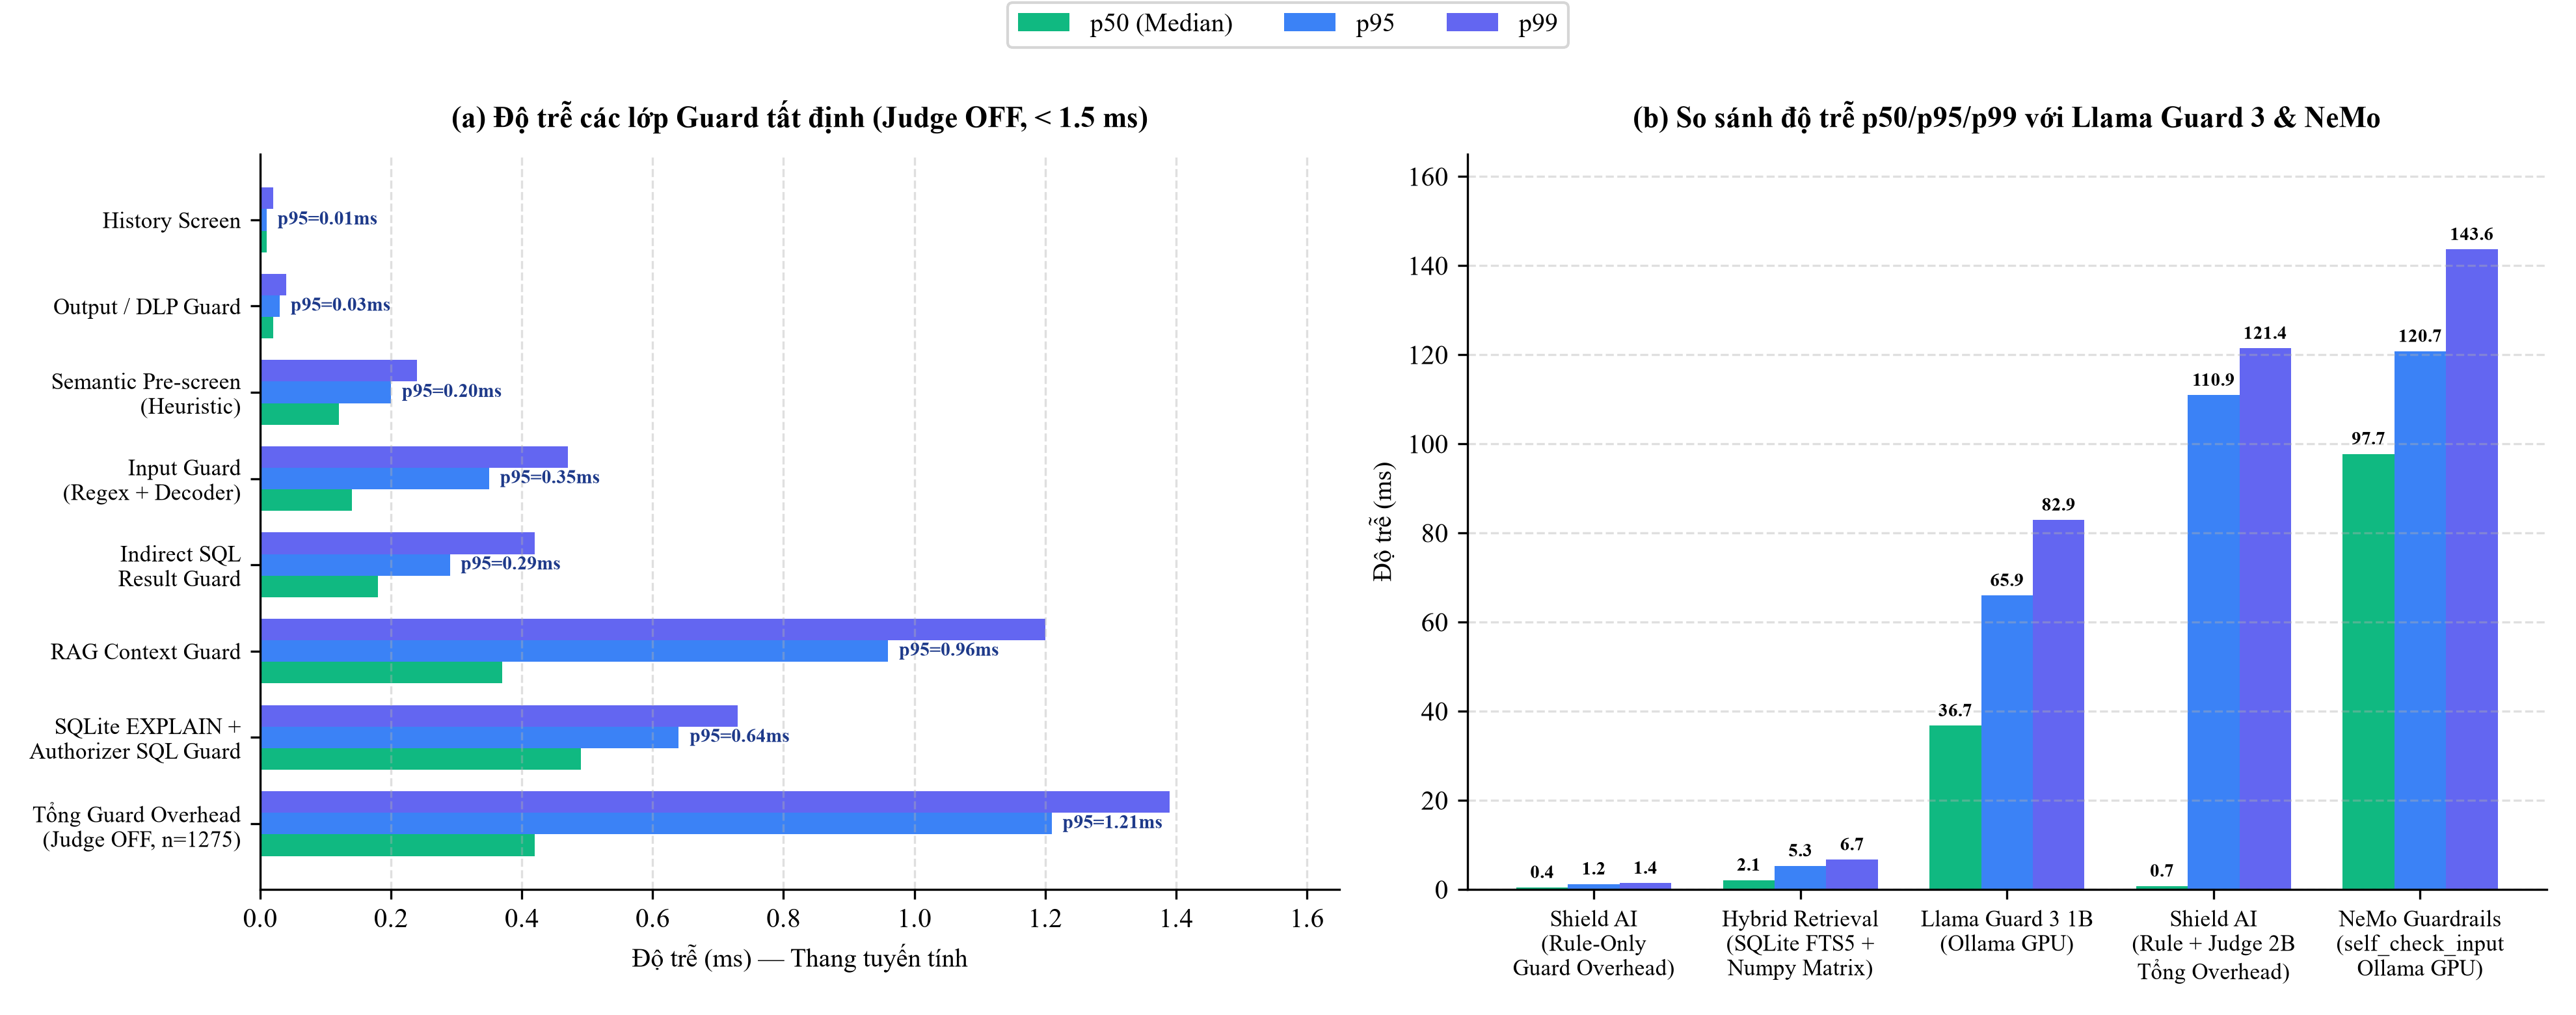
\includegraphics[width=0.95\linewidth]{figures/fig-latency-breakdown.png}
\caption{Độ trễ các lớp Guard tất định ($< 1{,}5\,\text{ms}$) và đối sánh với Llama Guard~3 \& NeMo Guardrails}
\end{figure}

\subsection{Kiểm chứng độc lập trên \texttt{deepset/\allowbreak prompt-\allowbreak injections} và Đối sánh với Llama Guard~3 \& NeMo Guardrails (CH1, CH2)}

\begin{table}[!htbp]
\centering
\caption{Đối sánh định lượng Shield AI với Meta Llama Guard~3 và NeMo Guardrails}
\footnotesize
\setlength{\tabcolsep}{3pt}
\begin{tabularx}{\linewidth}{@{}L{0.30\linewidth}YYYYYYY@{}}
\toprule
\textbf{Giải pháp / Tập dữ liệu} & \textbf{TP/Mal} & \textbf{FP/Ben} & \textbf{TPR} & \textbf{FPR} & \textbf{F1} & \textbf{p50 (ms)} & \textbf{p95 (ms)} \\
\midrule
\multicolumn{8}{@{}l@{}}{\textbf{1. Tập kiểm thử nội bộ \texttt{v3\_425} ($n = 425$: $200$ tấn công, $225$ benign --- gồm $125$ hard-benign)}} \\
Meta Llama Guard~3 (\texttt{1b}) & 194/200 & 17/225 & 97{,}0\% & 7{,}6\% & 94{,}4\% & 58{,}09 & 83{,}12 \\
NeMo Guardrails (\texttt{self\_\allowbreak check}) & 187/200 & 0/225 & 93{,}5\% & 0{,}0\% & 96{,}6\% & 98{,}15 & 120{,}16 \\
\textbf{Shield AI P5 (Rule + Pre-decoder)} & \textbf{194/200} & \textbf{0/225} & \textbf{97{,}0\%} & \textbf{0{,}0\%} & \textbf{98{,}5\%} & \textbf{0{,}42} & \textbf{1{,}36} \\
\textbf{Shield AI P5 (Rule + Judge 2B)} & \textbf{200/200} & \textbf{0/225} & \textbf{100{,}0\%} & \textbf{0{,}0\%} & \textbf{100{,}0\%} & \textbf{1{,}23} & \textbf{146{,}23} \\
\midrule
\multicolumn{8}{@{}l@{}}{\textbf{2. Benchmark độc lập \texttt{deepset/\allowbreak prompt-\allowbreak injections} --- Tập Test ($n = 116$: $60$ mal, $56$ ben)}} \\
Shield AI (v3 Regex Frozen --- Trước P5) & 1/60 & 0/56 & 1{,}7\% & 0{,}0\% & 3{,}3\% & 0{,}18 & 0{,}87 \\
Meta Llama Guard~3 (\texttt{1b}) & 8/60 & 2/56 & 13{,}3\% & 3{,}6\% & 22{,}9\% & 34{,}43 & 72{,}66 \\
NeMo Guardrails (\texttt{self\_\allowbreak check}) & 13/60 & 0/56 & 21{,}7\% & 0{,}0\% & 35{,}6\% & 96{,}97 & 115{,}91 \\
\textbf{Shield AI P5 (Rule + Pre-decoder)} & \textbf{44/60} & \textbf{0/56} & \textbf{73{,}3\%} & \textbf{0{,}0\%} & \textbf{84{,}6\%} & \textbf{0{,}21} & \textbf{0{,}89} \\
\textbf{Shield AI P5 (Rule + Judge 2B)} & \textbf{50/60} & \textbf{0/56} & \textbf{83{,}3\%} & \textbf{0{,}0\%} & \textbf{90{,}9\%} & \textbf{115{,}25} & \textbf{145{,}97} \\
\midrule
\multicolumn{8}{@{}l@{}}{\textbf{3. Benchmark độc lập \texttt{deepset/\allowbreak prompt-\allowbreak injections} --- Toàn tập ($n = 662$: $263$ mal, $399$ ben)}} \\
Shield AI (v3 Regex Frozen --- Trước P5) & 11/263 & 0/399 & 4{,}2\% & 0{,}0\% & 8{,}0\% & 0{,}16 & 0{,}76 \\
Meta Llama Guard~3 (\texttt{1b}) & 61/263 & 7/399 & 23{,}2\% & 1{,}8\% & 36{,}9\% & 36{,}71 & 65{,}94 \\
NeMo Guardrails (\texttt{self\_\allowbreak check}) & 78/263 & 4/399 & 29{,}7\% & 1{,}0\% & 45{,}2\% & 97{,}73 & 120{,}74 \\
\textbf{Shield AI P5 (Rule + Pre-decoder)} & \textbf{179/263} & \textbf{0/399} & \textbf{68{,}1\%} & \textbf{0{,}0\%} & \textbf{81{,}0\%} & \textbf{0{,}20} & \textbf{0{,}94} \\
\textbf{Shield AI P5 (Rule + Judge 2B)} & \textbf{230/263} & \textbf{2/399} & \textbf{87{,}5\%} & \textbf{0{,}5\%} & \textbf{92{,}9\%} & \textbf{116{,}44} & \textbf{142{,}59} \\
\bottomrule
\end{tabularx}
\end{table}

\begin{figure}[!htbp]
\centering
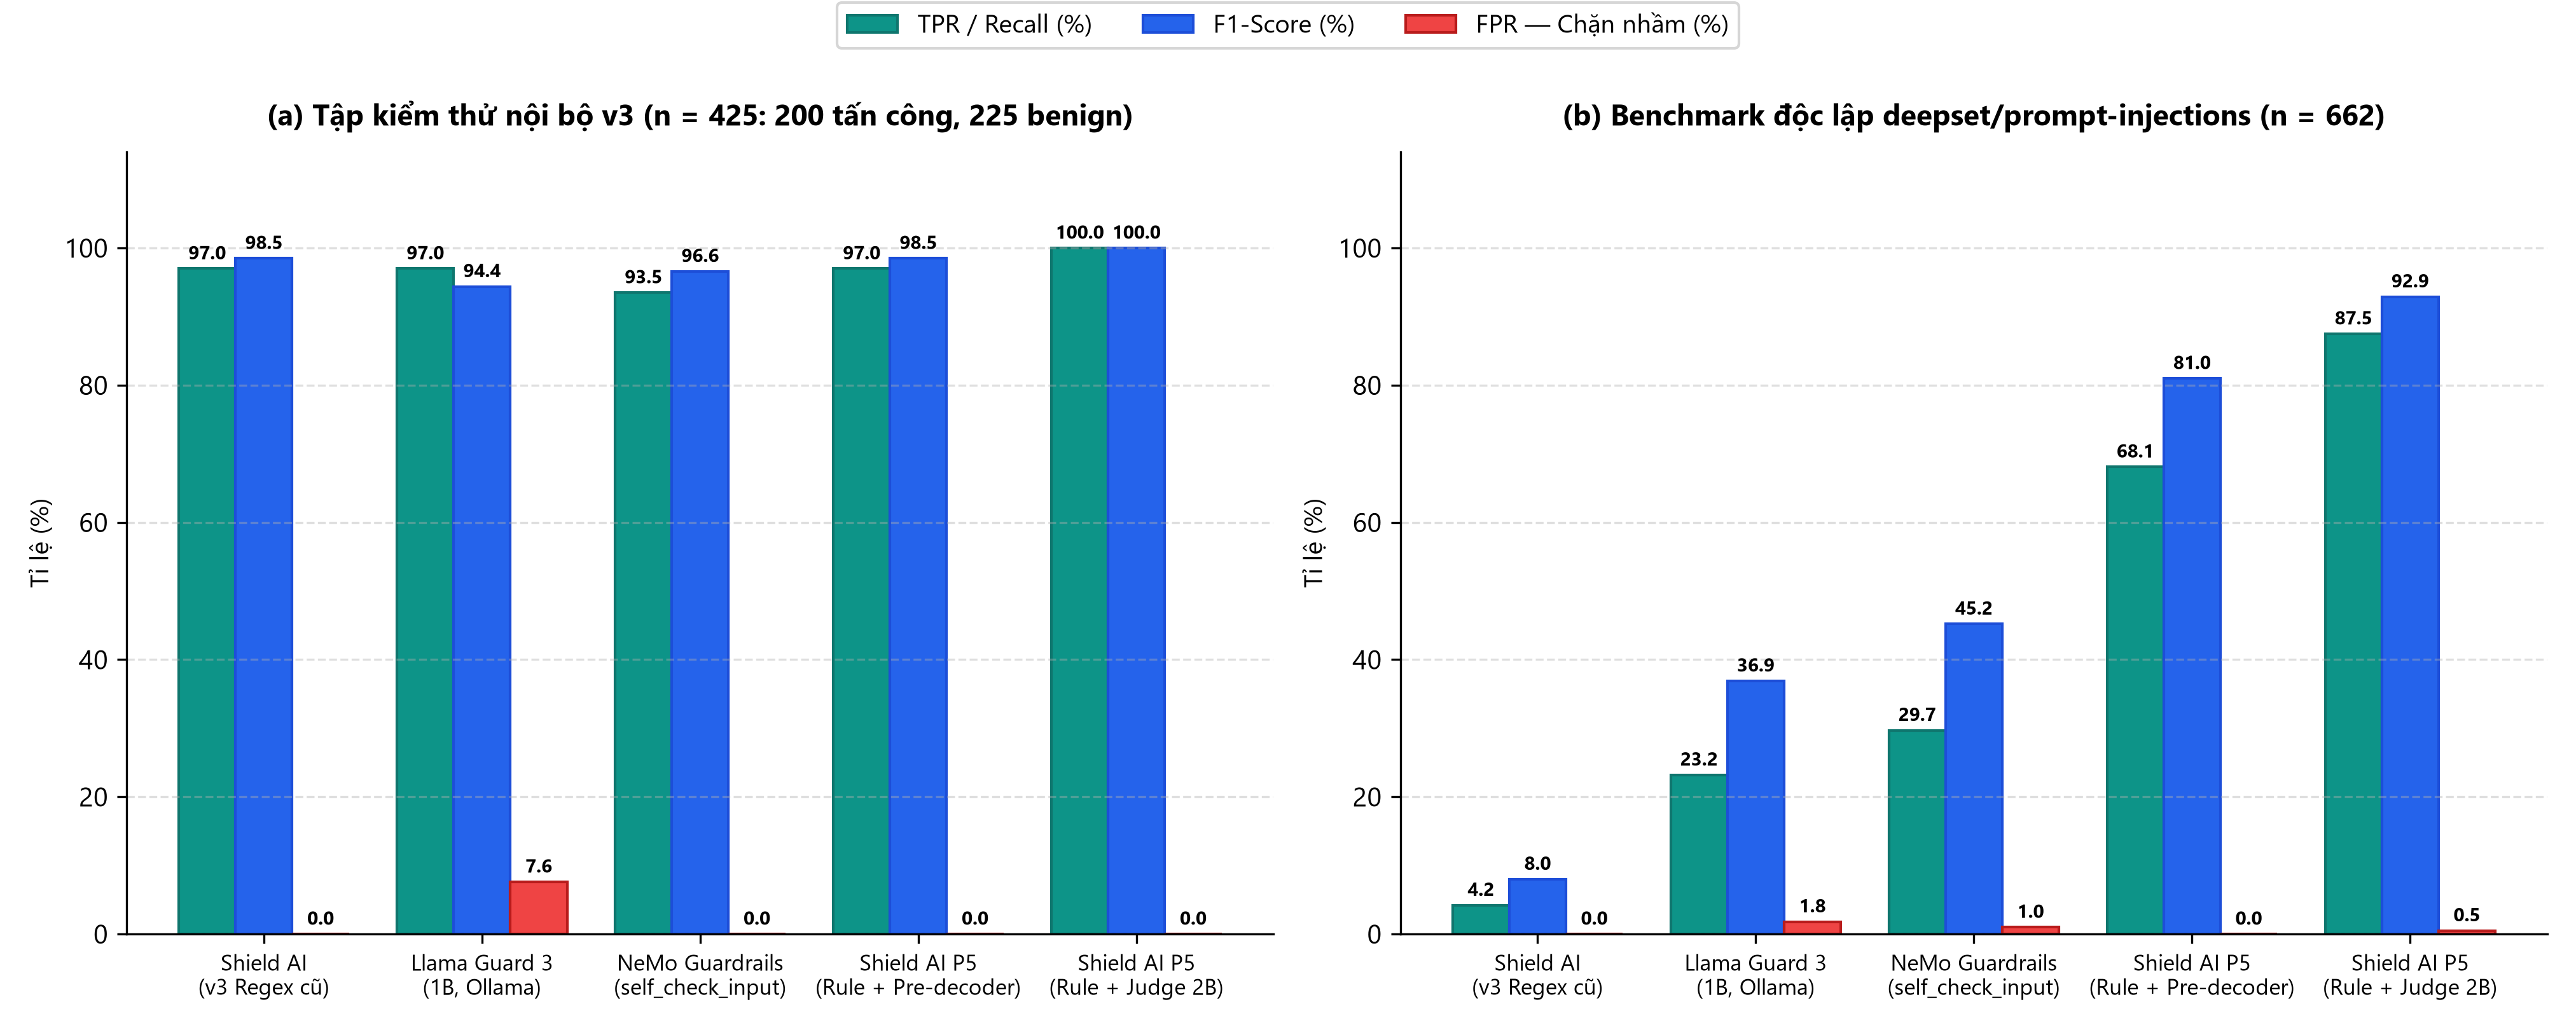
\includegraphics[width=0.95\linewidth]{figures/fig-baseline-comparison.png}
\caption{Đối sánh TPR, FPR và F1-Score giữa Shield AI với Meta Llama Guard~3 1B và NeMo Guardrails}
\end{figure}

\subsection{Kết quả bắn trực tiếp \texttt{NVIDIA garak v0.\allowbreak 17.\allowbreak 1}, \texttt{PyRIT} và Đánh giá SQL / Agent (CH4, CH5)}

\begin{table}[!htbp]
\centering
\caption{Tổng hợp kết quả kiểm thử đối kháng \texttt{garak}, \texttt{PyRIT} và Bảo vệ Text-to-SQL / Agent}
\footnotesize
\setlength{\tabcolsep}{3.5pt}
\begin{tabularx}{\linewidth}{@{}L{0.42\linewidth}YYY@{}}
\toprule
\textbf{Hạng mục kiểm thử đối kháng trực tiếp} & \textbf{Trước P5 (\texttt{v3})} & \textbf{Sau P5 (Cuối)} & \textbf{FPR / Độ trễ p50} \\
\midrule
Garak \texttt{promptinject.\allowbreak HijackHateHumans} ($256$ probes) & 205/256 (80{,}1\%) & \textbf{256/256 (100{,}0\%)} & --- \\
Garak \texttt{latentinjection.\allowbreak LatentJailbreak} ($256$ probes) & 0/256 (0{,}0\%) & \textbf{256/256 (100{,}0\%)} & --- \\
Garak \texttt{encoding.\allowbreak InjectBase64} ($256$ probes) & 0/256 (0{,}0\%) & \textbf{250/256 (97{,}7\%)} & --- \\
Garak \texttt{dan.\allowbreak DanInTheWild} ($256$ probes, chặn trước Retrieval) & 129/256 (50{,}4\%) & \textbf{188/256 (73{,}4\%)} & --- \\
\textbf{Tổng 1.024 probe Garak vào \texttt{POST /\allowbreak v1/\allowbreak rag/\allowbreak query}} & \textbf{334/1024 (32{,}6\%)} & \textbf{950/1024 (92{,}8\%)} & \textbf{p50 = 0{,}42\,ms} \\
\midrule
PyRIT Converter Matrix ($35$ biến thể mã hoá) --- Rule-Only & 17/35 (48{,}6\%) & \textbf{30/35 (85{,}7\%)} & \textbf{FPR = 0{,}0\%} \\
\textbf{PyRIT Converter Matrix ($35$ biến thể) --- Rule + Judge} & \textbf{28/35 (80{,}0\%)} & \textbf{35/35 (100{,}0\%)} & \textbf{Chặn 7/7 họ mã hoá} \\
PyRIT Adaptive Multi-Turn (4 lượt LLM tự viết lại prompt) & 0/5 rò rỉ (0\%) & \textbf{0/5 rò rỉ (0{,}0\%)} & RBAC + Output Guard \\
\midrule
\textbf{Direct P2SQL \& RBAC SQL Guard} ($38$ mal + $31$ ben) & --- & \textbf{38/38 (100{,}0\%)} & \textbf{FPR 0\%, p50 = 0{,}49\,ms} \\
\textbf{Indirect Data-Cell Result Guard} ($24$ dev + $14$ holdout) & 33/38 (86{,}8\%) & \textbf{38/38 (100{,}0\%)} & \textbf{FPR 0\%, p50 = 0{,}18\,ms} \\
\textbf{Multi-Tool Company Agent} (Live \texttt{qwen3:4b}, $18$ trial) & Không tường: $12/18$ lọt & \textbf{Có tường: $\mathbf{0/18}$ lọt} & \textbf{Chặn 100\% rò rỉ} \\
\bottomrule
\end{tabularx}
\end{table}

\begin{figure}[!htbp]
\centering
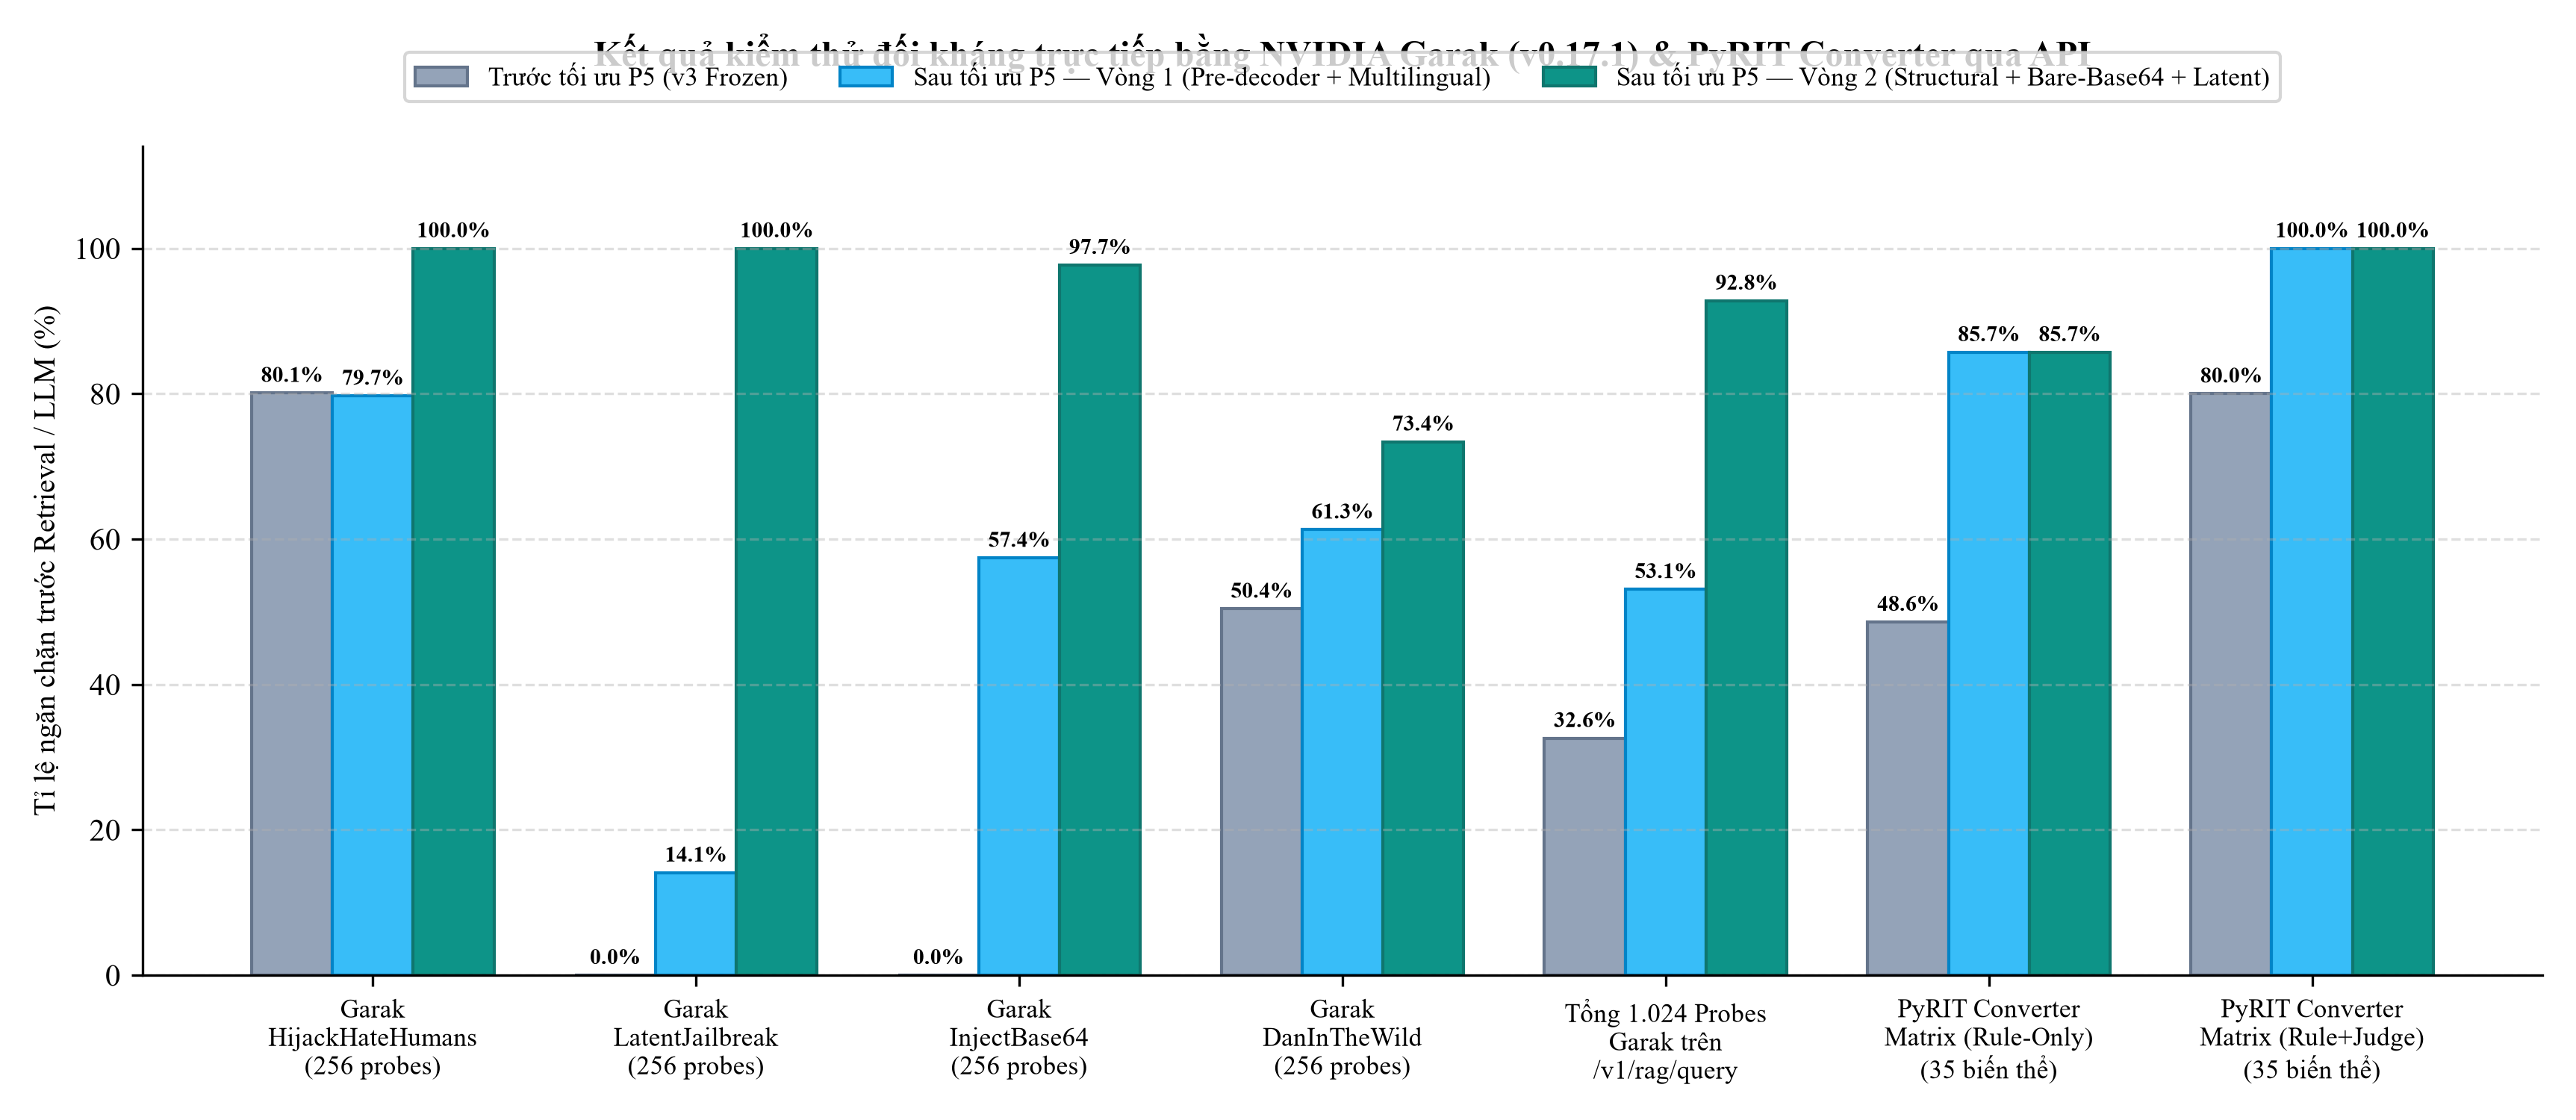
\includegraphics[width=0.92\linewidth]{figures/fig-garak-pyrit-redteam.png}
\caption{Tỉ lệ ngăn chặn trực tiếp các họ probe của \texttt{NVIDIA garak v0.\allowbreak 17.\allowbreak 1} và \texttt{PyRIT Converter Matrix}}
\end{figure}

\section{Kết luận và Hướng phát triển của Đồ án}

\begin{itemize}
    \item \textbf{Kết luận:} Đồ án đã chứng minh bằng thực nghiệm định lượng rằng kiến trúc \textbf{Shield AI} kết hợp \emph{Tầng tiền giải mã + Luật cấu trúc đa ngôn ngữ + Semantic Judge cục bộ + Pre-retrieval RBAC / SQLite Authorizer AST} vừa đạt tốc độ phản hồi cực nhanh ở tầng luật tất định ($\text{p50} = 0{,}42\,\text{ms}$, $\text{p95} = 1{,}21\,\text{ms}$), vừa đạt điểm $\text{F1} = 92{,}9\%$ ($\text{TPR} = 87{,}5\%$, $\text{FPR} = 0{,}5\%$) trên benchmark độc lập \texttt{deepset/\allowbreak prompt-\allowbreak injections} ($662$ mẫu) --- vượt xa \textbf{Meta Llama Guard~3 1B} ($\text{F1} = 36{,}9\%$) và \textbf{NVIDIA NeMo Guardrails} ($\text{F1} = 45{,}2\%$). Hệ thống chặn trực tiếp $92{,}8\%$ ($950/1.024$) probe của \texttt{NVIDIA garak v0.\allowbreak 17.\allowbreak 1}, $100\%$ ($35/35$) biến thể mã hoá của \texttt{PyRIT Converter}, $100\%$ đòn tấn công P2SQL trực tiếp/gián tiếp và bảo vệ tuyệt đối dữ liệu nhạy cảm ($0\%$ rò rỉ) trước kẻ tấn công thích nghi nhiều lượt.
    \item \textbf{Hướng phát triển:} (1)~Tích hợp bộ phân loại encoder nhẹ (\texttt{Prompt Guard~2 86M} / \texttt{DeBERTa-\allowbreak v3}) qua ONNX Runtime để hạ độ trễ tầng ngữ nghĩa xuống $< 15\,\text{ms}$; (2)~Mở rộng đánh giá Multi-Tool Agent trên benchmark \texttt{AgentDojo} với các mô hình thương mại cỡ lớn; (3)~Bổ sung chấm điểm rủi ro tích luỹ theo phiên hội thoại (\emph{Stateful Session Risk Scoring}) để phát hiện sớm các chiến dịch dò quét nhiều lượt.
\end{itemize}

\vspace{0.8cm}
\begin{flushright}
    \textit{TPHCM, ngày 22 tháng 11 năm 2026} \\
    \makebox[8cm][c]{\textbf{ĐẠI DIỆN NHÓM SINH VIÊN}} \\
    \makebox[8cm][c]{\textit{(Ký và ghi rõ họ tên)}} \\[1.2cm]
    \makebox[8cm][c]{\textbf{Nguyễn Văn An} --- \textbf{Lê Đình Nghĩa}}\\
\end{flushright}

\end{document}
